% !TEX program = xelatex
\documentclass[a4paper,10pt,twocolumn]{article}

% \usepackage[mongolian]{babel} 
\usepackage{fontspec}

\setmainfont{Times New Roman}
\newfontfamily\cyrillicfont{Times New Roman}[Script=Cyrillic]

\setmonofont{Courier New}
\newfontfamily\cyrillicfonttt{Courier New}[Script=Cyrillic]

\usepackage[top=0.5in, bottom=0.8in, left=0.87in, right=0.91in]{geometry}
\usepackage{titlesec}
\usepackage{indentfirst} 
\usepackage{float}

\usepackage{xcolor}        
\usepackage{colortbl}    
\usepackage{graphicx}
\usepackage{booktabs}
\usepackage{tabularx}
\usepackage{caption}

\usepackage{amsmath,amssymb}
\usepackage{listings}

\usepackage{hyperref}    
\usepackage{cleveref}    
\usepackage{caption}

\crefname{figure}{зураг}{зураг}
\crefname{table}{хүснэгт}{хүснэгт}

\crefformat{figure}{\textit{#2#1#3 - р зураг}}
\crefformat{table}{Хүснэгт. #2#1#3}

\definecolor{codebg}{RGB}{245,245,245}
\definecolor{codekey}{RGB}{0,0,160}
\definecolor{codecom}{RGB}{0,128,0}
\definecolor{tblheader}{RGB}{91,155,213}

\setlength{\columnsep}{0.25in}
\setlength{\parindent}{0.25in} 
\raggedbottom 
\pagestyle{empty} 

\renewcommand{\thesection}{\Roman{section}}
\titleformat{\section}[block]{\centering\normalfont\large\bfseries}{\thesection.}{0.5em}{}
\titlespacing{\section}{0pt}{12pt}{6pt} 

\renewcommand{\thesubsection}{\Alph{subsection}}
\titleformat{\subsection}[block]{\normalsize\itshape}{\thesubsection.}{0.5em}{}
\titlespacing{\subsection}{0pt}{10pt}{4pt}

\title{\fontsize{13.5pt}{16pt}\selectfont\textbf{\uppercase{qwen3.5-2B загварыг монгол өгөгдлөөр 4 шатаар сургах нь}}}

\renewcommand{\tablename}{Хүснэгт}
\DeclareCaptionLabelFormat{customtable}{#1. #2}
\DeclareCaptionLabelFormat{customfig}{#2 - р зураг}

\captionsetup[table]{
	labelformat=customtable, 
	labelsep=none,            
	justification=raggedleft, 
	singlelinecheck=false,    
	font=it                  
}

\captionsetup[figure]{
	labelformat=customfig,
	labelsep=space,
	font=it
}

\author{
	\parbox{\textwidth}{\centering \fontsize{9.5pt}{11pt}\selectfont
		\textbf{Бөхбатын Амартүвшин\textsuperscript{1}, Нямын Гантөмөр\textsuperscript{1}} \\[1ex]
		\textsuperscript{1}Монгол улс, Улаанбаатар, ШУТИС, Мэдээлэл холбооны технологийн сургууль, Компьютерын ухааны тэнхим \\
		%\textsuperscript{2}Монгол улс, Улаанбаатар, ШУТИС, Мэдээлэл холбооны %технологийн сургууль, Компьютерын ухааны тэнхим\\[1ex]
		\textit{\underline{B231910004@must.edu.mn}}\textsuperscript{1}, \textit{\underline{B231960002@must.edu.mn}}\textsuperscript{2}
	}
}

\date{}

\begin{document}
	\renewcommand{\tablename}{Хүснэгт} 
	\twocolumn[{
		\maketitle
		\thispagestyle{empty} 
		\vspace{-2em}
		
		\noindent
		\begin{minipage}{\textwidth}
			\fontsize{9pt}{11pt}\selectfont
			\textbf{\textit{Хураангуй:}} \textbf{Энэхүү курсын ажлын хүрээнд Qwen3.5-2B-Base суурь загварыг Монгол хэл дээрх өгөгдөл ашиглан Continued Pretraining, QA SFT, DPO, болон Instruction tuning гэсэн дөрвөн үе шаттайгаар сургав. Тухайн загварыг бүтнээр нарийн тохируулахад (Full-Fine tune) хийхэд тооцооллын нөөцийн хязгаарлалт үүссэн учир Unsloth сан болон QLoRA аргачлалыг AdamW оптимизатортай хослуулан ашигласан. Сургалтын эхний шатанд Монгол текст өгөгдлөөр урьдчилан сургалт хийж, загварын хэл зүйн бүтцийг ойлгох чадварыг сайжруулан Perplexity утгыг мэдэгдэхүйц багасгаж тогтворжуулсан. Хоёрдугаар шатанд асуулт хариултын өгөгдлийг ChatML форматаар сургаснаар F1 оноо зохих түвшинд хүрсэн. Гуравдугаар шатанд (DPO) хос өгөгдөл дээр сургахад баталгаажуулалтын алдаа багасаж, хүний хариултыг ялгах чадвар (Reward accuracy) өндөр хувьтай болсон бөгөөд эцсийн шатанд Tavily API ашиглан тусгайлан бэлтгэсэн өгөгдлөөр функц дуудах (function-calling) чадварыг суулгасан. Туршилтаар QLoRA нь график санах ойн зарцуулалтыг үр дүнтэй бууруулсан хэдий ч квантчлалын нөлөөгөөр үүсэх мэдээллийн алдагдал, DPO шатны хэт өндөр урамшууллын онооноос шалтгаалсан хэт цээжлэх (overfitting) эрсдэл зэрэг техникийн хязгаарлалтууд үүссэн болно.}
			
			\vspace{0.3cm}
			\textbf{\textit{Түлхүүр үг:}} \textbf{\textit{LLM, NLP, Qwen3.5-mn}}
		\end{minipage}
		\vspace{0.8cm}
	}]
	
	\section{Оршил}
	Том хэлний загвар (large language model) нь хэлний загварчлалын хамгийн боловсронгуй загвар юм. Энэ нь Статистик хэлний загвар (statistic language model), Мэдрэлийн сүлжээнд суурилсан хэлний загвар (neural language model), урьдчилагдан сургагдсан хэлний загваруудын (pre-trained language model) хувьслын үр дүнд бий болсон transformers архитектур дээр суурилсан нэгдсэн том систем юм. Тэрбумаас их наядаар хэмжигдэх параметр агуулсан загварууд нь асар их хэмжээний текст өгөгдөл дээр урьдчилан сургагдсан байдаг. Загвар нь текстийг боловсруулахдаа хамгийн түрүүнд үгсийг тасралтгүй вектор орон зайд хувиргаж, үг хоорондын утга зүйн хамаарлыг орон зайгаар тодорхойлдог механизмтай. Уламжлалт статистик , болон мэдрэлийн сүлжээнд суурилсан хэлний загваруудаас transformers архитектурын self-attention механизм ашиглан өгүүлбэр дэх үгс хоорондын зайны хамаарлыг зэрэгцээгээр тооцоолж, өмнөх агуулгад тулгуурлан дараагийн үгийн гарах магадлалын үржигдэхүүнийг урьдчилан таамаглах зарчмаар ажилладаг. 
	
	Энэхүү судалгааны ажилд суурь болгон ашигласан Qwen3.5-2B-Base загвар нь 2 тэрбум параметртэй, олон хэлний чадавх сайтай, нээлттэй эхийн том хэлний загвар бөгөөд текст үүсгэх, ойлгох, болон төрөл бүрийн хэл шинжлэлийн даалгавруудыг өндөр нарийвчлалтай гүйцэтгэх чадвартай юм \cite{qwen}. Уг загварыг суурь болгон ашиглах нь тооцооллын нөөцийн хязгаарлагдмал байдалд тохирохоос гадна Монгол хэлний онцлогт нийцүүлэн нэмэлт сургалт хийхэд оновчтой сонголт болдог.
	
	Transformers архитектурын давуу тал нь аливаа хэлний хэлбэр зүйн онцлогоос үл хамааран утга зүйн ижил төстэй байдлыг суралцах боломжийг олгодог. Гэсэн хэдий ч том хэлний загваруудын өвөрмөц хэв шинж, бүтэцтэй хэлнүүд дээр шууд Англи хэлтэй ижил хэмжээнд сайн суралцдаггүй бөгөөд архитектурын тодорхой хэмжээний тохируулга хийх шаардлагатай юм. 
	
	Монгол хэл нь Англи хэл зэрэг их нөөцтэй хэлнүүдтэй харьцуулахад дижитал өгөгдлийн хэмжээ харьцангуй маш бага нөөцтэй хэлний ангилалд багтдаг. Том хэлний загваруудыг урьдчилан сургахад асар их хэмжээний цэвэр өгөгдөл шаарддаг бол Монгол хэлний хувьд чанартай нээлттэй эхийн текст, асуулт хариултын төрөлжсөн өгөгдлийн сангууд хомс байдаг. Үүнээс гадна бүтцийн хувьд англи хэлтэй ижил тусгаарлах хэл биш, харин үгний үндэстэй дагавар, нөхцөл залгаж шинэ утга үүсгэдэг залгамал хэл учраас нэг язгуураас хэдэн зуун шинэ утга үүсэх боломжтой байдал нь үгийн сангийн хэмжээг маш ихээр нэмэгдүүлж токенжуулалтын шатанд хүндрэл үзүлдэг. 
	
	\section{Өгөгдлийн багц (Dataset)}
	
	Энэхүү курсын ажлын хүрээнд нийт 4 шатлалт сургалт хийсэн бөгөөд сургалт, баталгаажуулалт, тестийн багцуудын хэмжээ болон онцлогийг доор дурдав. Бүх өгөгдлийг HuggingFace \texttt{datasets} сангаар боловсруулж сургалтад ашигласан.
	
	\begin{table}[H]
		\centering
		\fontsize{8pt}{10pt}\selectfont
		\renewcommand{\arraystretch}{1.2} 
		
		\caption{}
		\vspace{-4pt}
		
		\begin{tabularx}{\linewidth}{>{\raggedright\arraybackslash}X c c c}
			\toprule
			\textbf{\textit{Өгөгдлийн багц}} & \textbf{\textit{Train}} & \textbf{\textit{Val}} & \textbf{\textit{Test}} \\
			\midrule
			Урьдчилсан сургалт (text\_data) & 60,000 & 785 & 1,000 \\
			QA Fine-Tuning (qa\_data) & 98,000 & 1,025 & 10,000 \\
			DPO (dpo\_data) & 7,496 & 625 & 1,874 \\
			Instruction tuning (instruction\_data) & 900 & 50 & 50 \\
			\bottomrule
		\end{tabularx}
		\label{table1}
	\end{table}
	
	\textbf{Pretraining өгөгдөл:} Загварт Монгол хэлний суурь мэдлэг суулгах зорилготой ба нийт 61,785 мөр өгөгдлөөс бүрдэх бөгөөд төгсгөл бүрд \texttt{<eos>} токен залгаж бэлтгэсэн.
	
	\textbf{QA Fine-Tuning өгөгдөл:} Асуултад бүтэцтэй, үнэн зөв хариулдаг болгох зорилгоор ChatML формат руу хөрвүүлэгдсэн. Сургалтын багц дахь текстийн дундаж урт нь 363 токен орчим байна.
	
	\textbf{DPO өгөгдөл:} QA test багцаас асуултуудыг авч, зөв хариултыг (chosen) албан ёсны хариултаар, харин буруу хариултыг (rejected) Stage-2 загвараар үүсгүүлэн бэлтгэсэн. Ижил төстэй хариултуудыг шүүж хассанаар нийт 9,995 хос өгөгдөл үлдсэн.
	
	\textbf{Instruction өгөгдөл:} Tavily веб хайлтын API ашиглан асуултуудад зориулсан хайлтын үр дүнгүүдийг нэгтгэн функц дуудах (function-calling) систем, хэрэглэгч, туслахын харилцан ярианы ChatML формат руу хөрвүүлэн бэлтгэсэн байна.
	
	\section{Арга Зүй}
	
	Бүх 4 шатны сургалтад Qwen3.5-2B-Base загвар дээр Unsloth сан \cite{unsloth} болон QLoRA (4-bit) аргыг \cite{qlora} ашигласан. Unsloth нь Transformers сан дээр суурилсан өндөр түвшний (high-level wrapper) сан бөгөөд санах ойн хэрэглээг оновчилж, сургалтын хурдыг мэдэгдэхүйц нэмэгдүүлэх замаар өндөр үр ашигтай сургах боломжийг олгодог \cite{unsloth}. LoRA-ийн тохиргоонд $r=16, \alpha=16$, dropout $0$ байх ба attention болон MLP давхаргуудыг сургасан. 
	
	QLoRA нь загварын параметрүүдийг квантчлалаар шахаж, зөвхөн бага хэмжээст нэмэлт матрицуудыг сургаснаар график санах ойн (VRAM) хэрэгцээг эрс багасган, тооцооллын үр ашгийг нэмэгдүүлдэг шийдэл юм \cite{qlora}. Бүх шатанд 8-bit AdamW оптимизатор болон cosine learning rate хуваарийг ашигласан бөгөөд gradient checkpointing-ийг санах ой хэмнэх зорилгоор идэвхжүүлсэн.
	
	\subsection{Pretraining}
	Загварт Монгол хэлний суурь мэдлэг олгох үргэлжилсэн сургалт (Continued pretraining) хийсэн. Сургалтын хурд (learning rate) $2 \times 10^{-4}$, багцын хэмжээ (effective batch size) 8, текстийн дээд урт 1024 байхаар тохируулж нийт 25,000 алхам сургасан. 
	
	\subsection{QA Fine-Tuning}
	Асуулт хариултын өгөгдөл дээр SFT (Supervised Fine-Tuning) хийсэн. Сургалтын хурдыг $5 \times 10^{-5}$ болон $3 \times 10^{-5}$ гэсэн хоёр өөр утгаар туршиж үзсэн бөгөөд багцын хэмжээг 8, текстийн уртыг 1024 байхаар тохируулан 3-4 epoch сургасан.
	
	\subsection{DPO}
	Загварын хариултын чанарыг сайжруулахын тулд DPO (Direct Preference Optimization) аргаар \cite{dpo} сургасан. DPO нь хүн шиг сэтгэх, зөв болон буруу хариултыг ялгах чадварыг урамшууллын загвар (reward model) ашиглахгүйгээр шууд оновчилж, хүний хүлээлтэд нийцсэн чанартай хариулт гаргах үйл явцыг тогтворжуулдаг аргачлал юм \cite{dpo}. DPO-ийн $\beta=0.1$ параметр ашигласан ба сургалтын хурд $5 \times 10^{-6}$, багцын хэмжээ 16 байхаар тохируулсан. Нийт 1500 алхам сургасан бөгөөд 1400-р алхам дахь загвар хамгийн бага баталгаажуулалтын алдаатай гарсан.
	
	\subsection{Instruction tuning}
	Загварт веб хайлт хийх (Function-calling) чадвар суулгах зорилгоор эцсийн шатны SFT хийсэн. Сургалтын хурд $2 \times 10^{-4}$, багцын хэмжээ 16, текстийн дээд урт 2048 тохиргоотойгоор 57 алхам (1 epoch) сургасан. 
	
	\section{Үр Дүн}
	
	Сургалтын 4 үе шатны ерөнхий хэмжигдэхүүнүүд болох нийт сургасан алхам, зарцуулсан хугацаа болон хүрсэн хамгийн бага алдааны (min loss) утгуудыг \cref{table_summary_metrics}-д нэгтгэн харуулав. Эхний хоёр шатны хувьд лог мэдээлэл бүрэн хадгалагдаагүй тул нарийвчилсан хугацаа болон алдааны тоон утгууд хүснэгтэд ороогүй болно. Харин DPO шатанд 1500 алхам сургахад 5.61 цаг зарцуулж, баталгаажуулалтын алдаа 0.0353 хүрч хамгийн сайн үр дүнг үзүүлсэн байна. Instruction tuning шатанд 57 алхам сургахад ердөө 7 орчим минут зарцуулсан хэдий ч алдаа буурсан үр дүнтэй байна. \cref{table_summary_metrics} - д нийт 4 шат сургалтуудын нийт алхам болон түүний харгалзах баталгаажуулалтын алдааг харуулж байна.
	
	\begin{table}[H]
		\centering
		\fontsize{8pt}{10pt}\selectfont
		\renewcommand{\arraystretch}{1.2} 
		\caption{}
		\begin{tabularx}{\linewidth}{
				>{\raggedright\arraybackslash}X 
				>{\centering\arraybackslash}X 
				>{\centering\arraybackslash}X 
				>{\centering\arraybackslash}X
			}
			\toprule
			\textbf{\textit{Сургалтын шат}} & \textbf{\textit{Нийт алхам}} & \textbf{\textit{Зарцуулсан хугацаа}} & \textbf{\textit{Хамгийн бага алдаа}} \\
			\midrule
			Pretraining & 25,000 & 48.6 цаг & 1.387 \\
			QA Fine-Tuning & 3-4 epoch & 54.9 мин & 0.7537 \\
			DPO & 1,500 & 5.61 цаг & 0.0353 \\
			Instruction tuning & 57 & 7.08 минут & 0.9470 \\
			\bottomrule
		\end{tabularx}
		\label{table_summary_metrics}
	\end{table}
	
	\subsection{Pretraining}
	Урьдчилсан сургалтын шатанд загвар нь өгөгдсөн текстээс Монгол хэлний зүй тогтол, үгийн сангийн бүтцийг амжилттай суралцсан байна. \cref{fig:step1_train_loss}-т харуулснаар сургалтын явцад алхам нэмэгдэх тусам сургалтын алдаа (train loss) тасралтгүй багассан байна. Үүнтэй уялдан \cref{fig:step1_eval_loss}-т баталгаажуулалтын алдаа (eval loss) мөн адил буурч байгаа нь загвар цээжилж (overfitting) биш, харин ерөнхийлж сурч байгааг баталж байна. Дараагийн үгийг таамаглах чадварыг илтгэх гол хэмжигдэхүүн болох Perplexity нь \cref{fig:step1_eval_perp}-т харуулснаар мөн буурч тогтворжсон байна. Энэхүү тогтвортой сургалтын явц нь \cref{fig:step1_learning_rate}-т дүрслэгдсэн cosine learning rate хуваарьтай шууд холбоотой бөгөөд сургалтын төгсгөл рүү хурдыг жигд бууруулсан нь алдааг илүү нарийвчлан багасгахад эерэг нөлөө үзүүлжээ.
	
	\begin{figure}[H]
		\centering
		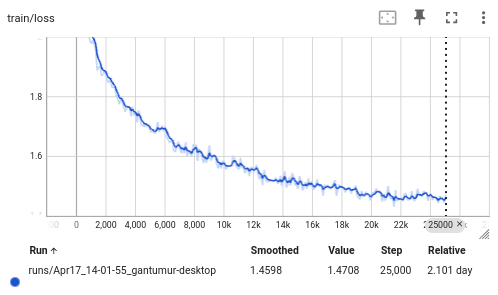
\includegraphics[width=0.98\linewidth]{images/step1_images/train_loss.png}
		\caption{Pretraining шатны сургалтын алдаа (Train loss)}
		\label{fig:step1_train_loss}
	\end{figure}
	
	\begin{figure}[H]
		
		\centering
		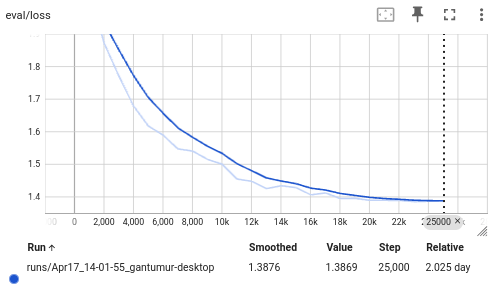
\includegraphics[width=0.98\linewidth]{images/step1_images/eval_loss.png}
		\caption{Pretraining шатны баталгаажуулалтын алдаа (Eval loss)}
		\label{fig:step1_eval_loss}
	\end{figure}
	
	\begin{figure}[H]
		\centering
		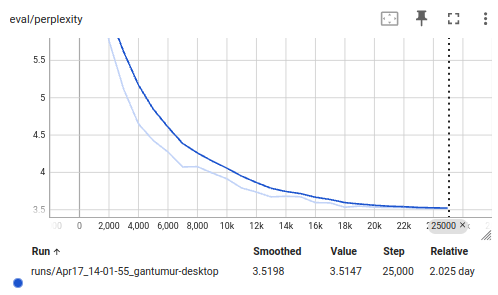
\includegraphics[width=0.98\linewidth]{images/step1_images/eval_perp.png}
		\caption{Pretraining шатны Perplexity}
		\label{fig:step1_eval_perp}
	\end{figure}
	
	\begin{figure}[H]
		\centering
		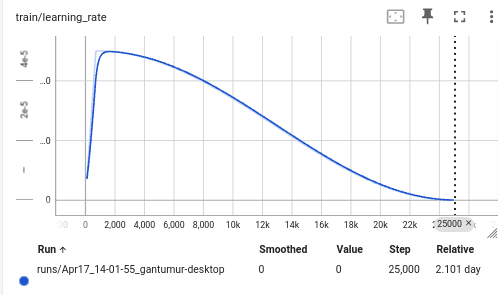
\includegraphics[width=0.98\linewidth]{images/step1_images/learning_rate.png}
		\caption{Pretraining шатны Learning rate}
		\label{fig:step1_learning_rate}
	\end{figure}
	
	\subsection{QA Fine-Tuning}
	Асуулт хариултын SFT шатны сургалтын үр дүнг \cref{fig:step2_train_loss} болон \cref{fig:step2_eval_loss}-т харуулсан ба сургалтын болон баталгаажуулалтын алдаа хоёулаа тогтвортой буурсан нь загвар асуулт хариултын форматад амжилттай дасан зохицож байгааг харуулж байна. Үүний зэрэгцээ асуулт хариултын системүүдийн чанарыг үнэлдэг гол хэмжигдэхүүнүүд болох Exact Match (EM) нь \cref{fig:step2_eval_em}-д, F1 оноо нь \cref{fig:step2_eval_f1}-д тус тус дүрслэгдсэн бөгөөд сургалтын алхам ахих тусам эдгээр оноонууд эрчимтэй өсөж, тодорхой түвшинд хүрээд тогтворжсон байна. Энэ нь загвар зөвхөн дүрэмзүйн хувьд зөв өгүүлбэр бүтээгээд зогсохгүй, хэрэглэгчийн асуултын гол утгыг ойлгож, зөвхөн оновчтой, яг таарсан мэдээллийг бүтэцлэгдсэн хэлбэрээр ялгаж хариулдаг болсныг нотолж байна.
	
	\begin{figure}[H]
		\centering
		
\includegraphics[width=0.98\linewidth]{images/step2_images/train_loss.png}
		\caption{QA шатны сургалтын алдаа (Train loss)}
		\label{fig:step2_train_loss}
	\end{figure}
	
	\begin{figure}[H]
		\centering
		
\includegraphics[width=0.98\linewidth]{images/step2_images/eval_loss.png}
		\caption{QA шатны баталгаажуулалтын алдаа (Eval loss)}
		\label{fig:step2_eval_loss}
	\end{figure}
	
	\begin{figure}[H]
		\centering
		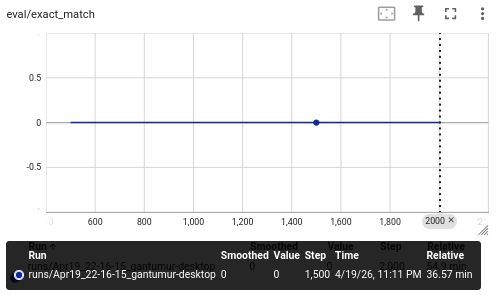
\includegraphics[width=0.98\linewidth]{images/step2_images/eval_exact_match.png}
		\caption{QA шатны Exact Match}
		\label{fig:step2_eval_em}
	\end{figure}
	
	\begin{figure}[H]
		\centering
		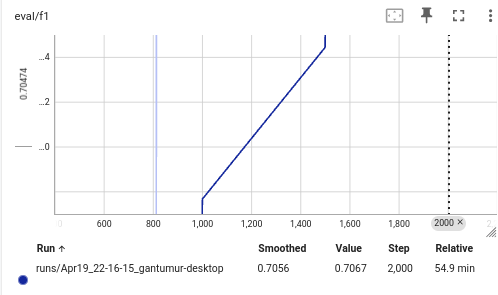
\includegraphics[width=0.98\linewidth]{images/step2_images/eval_f1.png}
		\caption{QA шатны F1 оноо}
		\label{fig:step2_eval_f1}
	\end{figure}
	
	\subsection{DPO}
	Нийт 1500 алхам сургахад \cref{fig:step3_train_loss}-т харуулснаар сургалтын алдаа (Train loss) 9.26-аас 0.003 хүртэл амжилттай буурч чадсан бөгөөд баталгаажуулалтын алдаа (Eval loss) нь \cref{fig:step3_eval_loss}-т харагдаж байгаачлан 1400-р алхамд хамгийн багадаа буюу 0.0353 хүрсэн нь хамгийн оновчтой цэг болсон байна. Үүний зэрэгцээ, загварын хүн шиг сэтгэх, зөв болон буруу хариултыг ялгах чадварыг илтгэх гол хэмжигдэхүүн болох Reward accuracy нь \cref{fig:step3_reward_acc}-д үзүүлснээр 0.9904 (99.04\%) хүрсэн нь маш өндөр бөгөөд амжилттай үр дүн юм. Мөн буруу эсвэл муу хариултыг гаргах магадлал болох Rejected logps нь \cref{fig:step3_logps_rejected}-д дүрслэгдсэнээр хүлээлтийн дагуу сургалтын явцад тогтмол буурсан байна. Энэ нь загвар хүний өгсөн чанартай хариултын хэв маягийг илүүд үзэж, алдаатай эсвэл хиймэл оюуны шинжтэй хариултуудаас амжилттай зайлсхийж сурсныг бүрэн харуулж байна.
	
	\begin{figure}[H]
		\centering
		
\includegraphics[width=0.98\linewidth]{images/step3_images/train_loss.png}
		\caption{DPO шатны сургалтын алдаа (Train loss)}
		\label{fig:step3_train_loss}
	\end{figure}
	
	\begin{figure}[H]
		\centering
		
\includegraphics[width=0.98\linewidth]{images/step3_images/eval_loss.png}
		\caption{DPO шатны баталгаажуулалтын алдаа (Eval loss)}
		\label{fig:step3_eval_loss}
	\end{figure}
	
	\begin{figure}[H]
		\centering
		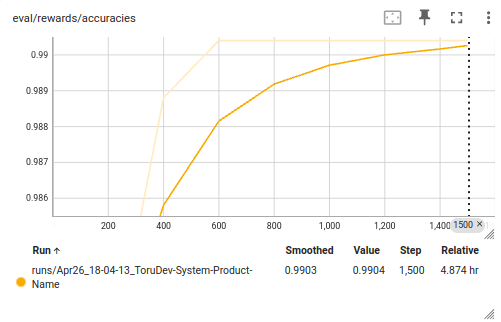
\includegraphics[width=0.98\linewidth]{images/step3_images/eval_reward_acc.png}
		\caption{DPO шатны Reward accuracy}
		\label{fig:step3_reward_acc}
	\end{figure}
	
	\begin{figure}[H]
		\centering
		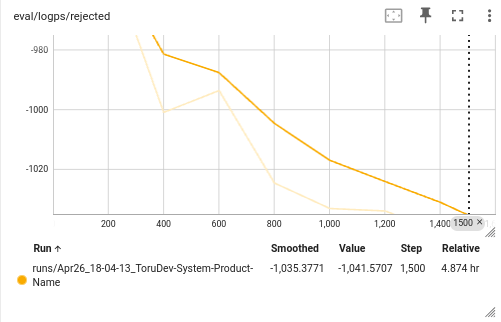
\includegraphics[width=0.98\linewidth]{images/step3_images/eval_logps_rejected.png}
		\caption{DPO шатны Rejected logps}
		\label{fig:step3_logps_rejected}
	\end{figure}
	
	\subsection{Instruction tuning}
	Нийт 57 алхам буюу 1 epoch сургахад \cref{fig:step4_train_loss}-т харуулснаар сургалтын алдаа 1.55-аас 0.96 болж хурдацтайгаар буурсан. Мөн \cref{fig:step4_eval_loss}-аас харахад баталгаажуулалтын алдаа (eval loss) сургалтын төгсгөлд 0.947 хүрсэн байна. Хэдийгээр харьцангуй цөөн алхам сургасан ч энэхүү хурдацтай алдааны бууралт нь функц дуудах (function-calling) болон веб хайлт хийж хариулах гэх мэт тусгайлсан зааварчилгааг ойлгох шинэ чадварыг загварт амжилттай суулгаж чадсаныг харуулж байна. Загвар нь хэрэгцээт мэдээллээ API-аар дамжуулан дуудаж, түүний үр дүнд тулгуурлан Монгол хэлээр эцсийн хариулт гаргах процессийг богино хугацаанд сайн эзэмшсэн.
	
	\begin{figure}[H]
		\centering
		
\includegraphics[width=0.98\linewidth]{images/step4_images/train_loss.png}
		\caption{Instruction tuning шатны сургалтын алдаа (Train loss)}
		\label{fig:step4_train_loss}
	\end{figure}
	
	\begin{figure}[H]
		\centering
		
\includegraphics[width=0.98\linewidth]{images/step4_images/eval_loss.png}
		\caption{Instruction tuning шатны баталгаажуулалтын алдаа (Eval loss)}
		\label{fig:step4_eval_loss}
	\end{figure}
	
	DPO болон Instruction tuning үе шатуудын сургалтын тодорхой алхмууд дахь алдааны утгуудыг \cref{table_loss_steps}-д харуулав. Хэдийгээр эхний хоёр шатны дата хэмжигдэхүүнүүд нь зөвхөн графикаар дүрслэгдсэн ч DPO болон Instruction шатуудын алдааны өөрчлөлтийг хүснэгтээр нэгтгэн харуулах нь загварын хэрхэн хурдан суралцсаныг харах боломж олгож байна.
	
	\begin{table}[H]
		\centering
		\fontsize{8pt}{10pt}\selectfont
		\renewcommand{\arraystretch}{1.2} 
		\caption{}
		\begin{tabularx}{\linewidth}{>{\raggedright\arraybackslash}X c c}
			\toprule
			\textbf{\textit{Алхам (Step)}} & \textbf{\textit{Train Loss}} & \textbf{\textit{Eval Loss}} \\
			\midrule
			\multicolumn{3}{c}{\textbf{Stage 3: DPO}} \\
			\midrule
			200  & 0.1608 & 0.1331 \\
			600  & 0.0130 & 0.0456 \\
			1000 & 0.0012 & 0.0357 \\
			1400 & 0.0012 & 0.0353 \\
			1500 & 0.0030 & 0.0356 \\
			\midrule
			\multicolumn{3}{c}{\textbf{Stage 4: Instruction Tuning}} \\
			\midrule
			10 & 1.5556 & - \\
			20 & 1.0985 & 1.0231 \\
			40 & 0.9959 & 0.9581 \\
			50 & 0.9691 & - \\
			57 & - & 0.9470 \\
			\bottomrule
		\end{tabularx}
		\label{table_loss_steps}
	\end{table}

	\section*{Дүгнэлт}
	Энэхүү курсын ажлаар Qwen3.5-2B-Base загварыг Монгол хэлний онцлогт тохируулан 4 үе шаттайгаар (Continued Pretraining, QA SFT, DPO, Instruction tuning) амжилттай сургаж, асуулт хариултын оновчтой систем болон веб хайлтад тулгуурласан функц дуудах (function-calling) чадвартай болгож чадлаа. 
	
	Сургалтын үр дүнгээс харахад үе шат бүрд сургалтын болон баталгаажуулалтын алдаа тодорхой хэмжээнд буурсан нь сургалтууд амжилттай явагдсаныг илэрхийлж байна. Жишээлбэл DPO сургалтын шатанд reward accuracy 99.04\%-д хүрч, загвар хүний өгсөн чанартай хариултыг амжилттай ялгаж сурсан байна. Мөн QA SFT шатанд Exact Match тохиолдоогүй боловч F1 оноо, Pretraining шатанд perplexity тус тус тогтвортой сайжирсан.
	
	Техникийн хэрэгжилтийн хувьд QLoRA (Quantized Low-Rank Adaptation) аргыг ашигласан нь хэд хэдэн чухал давуу талтай бөгөөд QLoRA нь үндсэн загварын параметрүүдийг 4-bit хэлбэрт шилжүүлж, зөвхөн нэмэлт бага хэмжээст LoRA  матрицуудыг сургаснаар VRAM-ийн зарцуулалтыг эрс багасгаж, хязгаарлагдмал тооцоолох хүчин чадалтай төхөөрөмж дээр том хэлний загварыг үр дүнтэй сургах боломжийг олгосон. Мөн Unsloth сангийн тусламжтайгаар сургалтын хурдыг нэмэгдүүлж, санах ойн хэрэглээг оновчилсон нь практик ач холбогдолтой байв.
	
	Гэсэн хэдий ч QLoRA нь зарим сул талуудтай болохыг туршилт харуулж байна. Квантчлалын (quantization) улмаас загварын нарийвчлалд бага зэргийн мэдээллийн алдагдал үүсэх эрсдэлтэй бөгөөд бүрэн параметрийн (full-parameter) сургалттай харьцуулахад шинэ мэдлэгийг сурах чадвар нь хязгаарлагдмал байх талтай. Түүнчлэн DPO сургалтын шатанд хэт өндөр reward гарсан нь загвар тодорхой өгөгдөл дээр хэт цээжлэх (overfitting) хандлагатай байж болзошгүйг харуулж байгаа тул цаашид илүү олон төрлийн, тэнцвэртэй өгөгдөл ашиглах шаардлагатайг илэрхийлж байна.
	
	Цаашдын ажилд илүү их хэмжээний цэвэр Монгол хэлний корпус ашиглан урьдчилсан сургалт хийх, гиперпараметрүүдийг (жишээлбэл: learning rate хуваарь, багцын хэмжээ) илүү нарийвчлан тохируулах, түүнчлэн QLoRA-ийн оронд өөр бусад параметр-хэмнэлттэй аргуудыг (PEFT) туршиж харьцуулах зэрэг нь загварын чадавхыг улам сайжруулах боломжтой юм.
	
	\renewcommand{\refname}{Ашигласан материал}
	
	\begin{thebibliography}{9}
		\bibitem{qwen}
		Bai, J., et al. "Qwen technical report." \textit{arXiv preprint arXiv:2309.16609} (2023).
		
		\bibitem{unsloth}
		Unsloth. "Unsloth: Fast LLM Training." \url{https://github.com/unslothai/unsloth} (2023).
		
		\bibitem{qlora}
		Dettmers, T., Pagnoni, A., Holtzman, A., \& Zettlemoyer, L. "QLoRA: Efficient Finetuning of Quantized LLMs." \textit{Advances in Neural Information Processing Systems}, 36 (2024).
		
		\bibitem{dpo}
		Rafailov, R., Sharma, A., Mitchell, E., Manning, C. D., Ermon, S., \& Finn, C. "Direct Preference Optimization: Your Language Model is Secretly a Reward Model." \textit{Advances in Neural Information Processing Systems}, 36 (2024).
	\end{thebibliography}

\end{document}